\section{Background}
\label{sec:background}

Radio searches for technosignatures began at centimetre wavelengths and
have largely stayed there. The first targeted experiments
\citep{CocconiMorrison1959,Drake1960}, the programmes reviewed by
\citet{Tarter2001} and Project Phoenix \citep{Backus2002} all worked
below a few gigahertz. The modern generation divides into targeted and
commensal surveys at centimetre and metre wavelengths
\citep{Zhang2020,Czech2021,FAST3IATLAS2025,LOFARdualsite2023,Choza2024},
several of them riding back-ends built for other science
\citep{Morrison2023}, with wide-field low-frequency coverage from the MWA
\citep{Tremblay2024}
and single-dish C- and K-band work at 6 and 18\,GHz with the Sardinia
Radio Telescope \citep{SRT2025}. Machine-learning interference rejection
is now central to that effort
\citep{Ma2023,GLOBULAR2025,AnomalyParkesGBT2025}. The classical threshold
search used here lacks that capability and instead uses a spatial test on
the star against control positions in the same field, which a single dish
cannot make. A narrowband search also reaches only one class of signal:
broadband planetary-scale leakage \citep{BRaTs2026} is outside it by
construction.

Above about 30\,GHz the record is nearly empty, and that is what makes
this frequency range new. ALMA's \SbNBand{} receiver bands cover
\SbBandLoGHz{} to \SbBandHiGHz\,GHz, and \SbNPriorBandWord{} of them has
been searched for technosignatures. The lowest,
\SbBandOneLoGHz--\SbBandOneHiGHz\,GHz, does hold observations of
\SbBoneNStar{} stars of this sample, but all from \SbBoneNProgWord{}
programme, all in a
continuum mode whose \SbBoneChanMHz\,MHz channels are \SbBoneChanRatio{}
times coarser than the narrowest channel searched here, and all
proprietary until \SbBoneRelYear: the coverage exists and cannot carry a
carrier search. The band above it holds none at all. For continuity with
the centimetre literature, the Arecibo planetary radar radiated
$\AreciboW$\,W at \ArecGHz\,GHz \citep{EarthDetectingEarth2025}; an
aperture of that diameter is not realisable in the millimetre band, so the
illustrative benchmark of \S\ref{sec:excludes} is instead a dish of
\BenchDiam\,m. The limits of this paper are stated as EIRP and need no
transmitter model.

\citet{Mason2025} is the only prior millimetre search of comparable bandwidth
and the only comparable archival one; the earlier nearby-star searches of
\citet{Steffes1994} and \citet{Mauersberger1996} covered a single line. They searched Band~3 windows toward
\MasonNStar{} Gaia~DR3 stars lying in the fields of \MasonNCal{} ALMA
calibrators, observed for other science and so usable for free. Their
nearest target is at \MasonNearKpc\,kpc, where a $5\sigma$ flux threshold
corresponds to EIRP$_{\rm min}>{}$\MasonNearEirp\,W. That target lies
between \MasonDistRatioFar{} and \MasonDistRatioNear{} times further away
than the stars searched here, so at a fixed received flux an EIRP ratio
between the two surveys would be
\MasonEirpOrdLo--\MasonEirpOrdHi{} orders of magnitude of $d^{2}$ and
almost nothing else. The quantity
that does not depend on distance is the minimum detectable \emph{received}
flux, $F_{\rm min}=S_{\rm min}\,\delta\nu$, and it has to be compared at
the channel width each experiment recorded: $S_{\rm min}$ falls as
$\delta\nu^{-1/2}$ while $F_{\rm min}$ rises as $\delta\nu^{1/2}$, so
putting a coarse window on a fine channel arithmetically credits it with a
depth it never reached. Mason
et~al.\ reach \MasonFluxLo--\MasonFluxHi\,W\,m$^{-2}$ across their four
fields, on a \MasonChanKHz\,kHz channel at a bare $5\sigma$ flux
threshold. On that same threshold convention and on native channels
throughout, the windows searched here reach \FluxTrigBest\,W\,m$^{-2}$ at
best --- a factor \FluxNatBestRatio{} deeper, in a channel
\FluxChanBestKHz\,kHz wide --- and \FluxTrigMed\,W\,m$^{-2}$ at the
median, a factor \FluxNatMedRatio{} shallower in a channel
\FluxChanMedKHz\,kHz wide. Per channel this survey is therefore the
shallower of the two except in its finest windows, and its advantage lies
elsewhere: \NSysClassA{} stellar systems within 40\,pc rather than distant
stars in four calibrator fields, and a frequency range reaching about nine
times higher. Mason et~al.\ also
identified the obstacles that shape the present method: drift rates scale
with frequency, smearing erodes sensitivity unless drift is searched for,
and the molecular line forest raises the confusion background. Every
window reported here was re-reduced and re-searched from the raw archive
with the pipeline of \S\ref{sec:method}.

Figure~\ref{fig:context}(a) places this survey among published searches,
in minimum detectable EIRP against distance. For a carrier narrower than
every programme's channel that limit is a total radiated power rather than
a spectral power density, so the axis is commensurable. The detection
thresholds behind the published limits are not: of the \LtNProg{}
programmes drawn, \LtNRescaled{} quote their limits at a threshold other
than $\LtCommonSnr\sigma$, and the minimum detectable flux is linear in
that threshold in each of their own expressions for it. Table~\ref{tab:litthresh}
gives each programme's threshold, the factor that puts it on the common
$\LtCommonSnr\sigma$ basis and the channel width it used, and the figure is
drawn after that rescaling, with each published value kept beside it. The
survey's own filled symbols are bare $\LtCommonSnr\sigma$ thresholds on the
same convention; the open symbols above them are $\mathrm{EIRP}_{90}$, the
power recovered nine times in ten through the single-epoch trigger stage,
and every limit in this paper is quoted on that. Any EIRP advantage toward
the nearest systems is a $d^{2}$ effect and not an instrumental one.
Panel~(b) is the other axis, the native channel width of every window
searched here beside the channel of each comparison programme. What
distinguishes this survey is its frequency range and the proximity of its
targets, not its depth in any one channel.

\begin{table}
\centering
\caption{The comparison programmes of Figure~\ref{fig:context}, each on its
own detection threshold and on the common $\LtCommonSnr\sigma$ basis.
$\mathrm{EIRP}_{\rm min}$ is the deepest limit each paper reports, and the
factor is $\LtCommonSnr/(\mathrm{S/N})$, the minimum detectable flux being
linear in the threshold in every one of their own expressions for it.}
\label{tab:litthresh}
\scriptsize
\setlength{\tabcolsep}{4pt}
%% GENERATED by make_fig_context_v410.py -- do not hand-edit.
\begin{tabular}{@{}lccccc@{}}
\toprule
programme & S/N & factor & $\Delta\nu_{\rm ch}$ & EIRP$_{\rm min}$ & at $5\sigma$ \\
 & & & & (W) & (W) \\
\midrule
Enriquez\,+\,17 & 25 & 0.20 & 2.8\,Hz & $10^{13}$ & $2\times10^{12}$ \\
Margot\,+\,23 & 10 & 0.50 & 3.0\,Hz & $1.35\times10^{13}$ & $6.75\times10^{12}$ \\
Price\,+\,20 & 10 & 0.50 & 2.8\,Hz & $2\times10^{12}$ & $10^{12}$ \\
Mason\,+\,25 & 5 & 1.00 & 30.5\,kHz & $6.91\times10^{17}$ & $6.91\times10^{17}$ \\
\bottomrule
\end{tabular}

\end{table}

\begin{figure}
\centering
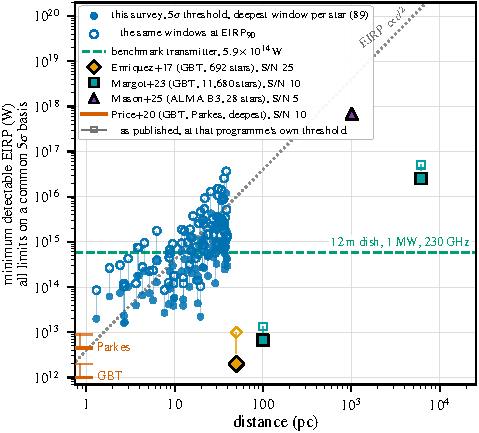
\includegraphics[width=\columnwidth]{figures/eirp_context_a.pdf}\\
{\footnotesize (a)}\\[4pt]
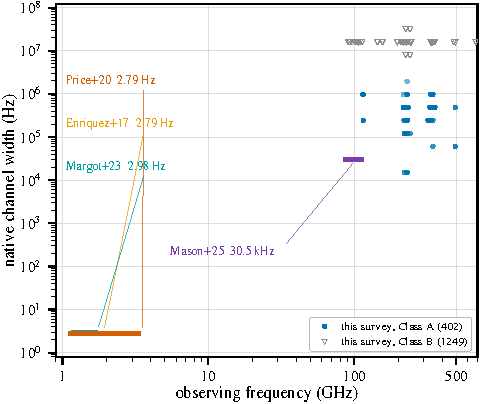
\includegraphics[width=\columnwidth]{figures/eirp_context_b.pdf}\\
{\footnotesize (b)}
\caption{Where this survey sits among published radio technosignature
searches. Every limit plotted is a total-power limit for a signal narrower
than the native channel of the experiment that set it. Those channels
differ by \LtChanSpanDex{} orders of magnitude, from \LtChanNarrow{} to
\LtChanWide, so the programmes are sensitive to different classes of
spectral feature and a signal detectable by one of them need not be
detectable by another at any power.
\textbf{(a)} Minimum detectable EIRP against distance, all on a common
$\LtCommonSnr\sigma$ basis. Blue, this survey, the deepest window per star:
\emph{filled}, that window's bare $\LtCommonSnr\sigma$ threshold;
\emph{open}, the same window at $\mathrm{EIRP}_{90}$, the single-epoch
trigger completeness of \S\ref{sec:pninetysel}, joined to its own
filled symbol. Orange, \citet{Enriquez2017}; aqua, \citet{Margot2023};
violet, \citet{Mason2025}; left-edge ticks, \citet{Price2020}. Each of
these is drawn at its published limit rescaled to $\LtCommonSnr\sigma$ by
the factor in Table~\ref{tab:litthresh}, with the published value itself as
the hollow marker joined above it. Grey dotted, EIRP $\propto d^{2}$ at
constant received flux; green dashed, the illustrative \BenchDiam\,m
benchmark transmitter of \S\ref{sec:excludes}. No symbol in the panel
carries a confirmation criterion.
\textbf{(b)} Native channel width against observing frequency for every
searched window (filled, Class~A; open, Class~B), with the comparison
programmes as horizontal segments at the widths of
Table~\ref{tab:litthresh}.}
\label{fig:context}
\end{figure}

A non-detection becomes a quantitative statement only through a stated
search volume. \citet{Wright2018} formalised that volume, and
\citet{Margot2023} its conversion into an upper bound on the fraction of
stars hosting a transmitter; \citet{EarthDetectingEarth2025} asked where
Earth's own technosignatures would be detectable. Such a bound is valid
only if the sample represents the population it is meant to describe.
This sample was assembled by other observers for other purposes, so it
does not, and \S\ref{sec:sample} states what it is instead.

%% Glenn's instruction, verbatim: the appendices are deliberately detailed and the
%% paper says so, so that a reader meets them as intended rather than as padding.
Because of the very specific and detailed statistical nature of this study, we have
extended the paper to include several very detailed Appendices that rigorously
explain the methodology involved.

%% Housekeeping. The two-symbol request on panel (a) -- bare 5 sigma filled,
%% EIRP_90 open, joined -- is satisfied by make_fig_context_v410.py and by the
%% caption above, so the standing note it carried is closed and deleted.
%% The Mason comparison is made here and nowhere else, now at NATIVE channel
%% widths on both sides: F_min propto dnu^(1/2), so rescaling our 488 kHz
%% median window to their 30.52 kHz flattered it by the square root of the
%% ratio (x4), which is a resolution app_A says no reprocessing can recover.
%% masoncmp_v401.py asserts that the two median comparisons differ by exactly
%% that square root, so the rescaled figures cannot be quoted again by
%% accident. The benchmark is evaluated once, in \S\ref{sec:excludes}, and is
%% labelled illustrative in both places it is named.
